\chapter{Resultados}
\label{cap:resultados}

En este capítulo se describe la aplicación del método de trabajo presentado en el capítulo \ref{cap:MiMetodologia} usando la metodología \gls{pud} en este caso concreto, mostrando los elementos (modelos, diagramas, especificaciones, etc.) más importantes y cómo satisface los objetivos y requisitos planteados.

También se explica la evolución de esta aplicación, desde la captura de requisitos hasta el resultado final.

\section{Arquitectura de la aplicación}
Para construir la arquitectura de la aplicación se ha optado por un modelo mixto Vista-Controlador, donde las capas que contienen los controladores y los objetos se conectan con la base de datos, y la capa con las interfaces, hace llamadas a los controladores y objetos para operar con ella.

\begin{itemize}
	\item \textbf{Capa de vistas:} esta capa representa las interfaces del programa.
	\item \textbf{Capa de controladores:} esta capa se comunica con la base de datos, y hace operaciones utilizando la capa de objetos.
	\item \textbf{Capa de objetos:} esta capa se comunica con la base de datos. Contiene todos los objetos del programa.
\end{itemize}

Se es consciente de que, si fuera un modelo vista-controlador puro, los controladores no deberían acceder a la base de datos. Esto se ha permitido por, entre otras cosas, permitir un nivel mayor de optimización en el código del que se habla en \ref{sub:optimizarcodigo}

En este documento, se refiere como único usuario al maestro que usará la aplicación.


\section{Requisitos del sistema}
A continuación se muestran los requisitos funcionales y no funcionales del sistema junto a una breve descripción.

\subsection{Requisitos funcionales}
Se han dividido los requisitos funcionales según el método descrito en la sección \ref{sub:obtencionrequisitos}.

Requisitos \textit{Must have}:
\begin{itemize}
	\item \textbf{MH1 - Asignación de asignaturas al usuario:} cada usuario tendrá asignadas las asignaturas de las que es titular durante el curso. 
	\item \textbf{MH2 - Creación de pruebas:} el usuario podrá crear pruebas en las diferentes asignaturas de las que es titular y asignarlas a un número de alumnos.
	\item \textbf{MH3 - Borrado de pruebas:} el usuario podrá borrar una prueba previamente creada, así como las notas de los alumnos que ya hayan sido calificados en esa prueba.
	\item \textbf{MH4 - Calificación de pruebas:} el usuario podrá calificar a los alumnos en las pruebas que cree para ellos. La calificación requiere una nota, y un comentario sobre la nota en caso de que el usuario requiera hacer alguna explicación.
	\item \textbf{MH5 - Visualización de las notas del alumnado:} el usuario debe poder visualizar las notas que ha calificado, así como las notas finales de cada trimestre y la nota final de la asignatura, para cada alumno.
	\item \textbf{MH6 - Visualización del alumnado para cada asignatura:} el usuario podrá ver un listado de los alumnos que corresponden a cada asignatura.
	\item \textbf{MH7 - Sistema de inicio de sesión para el usuario:} el usuario podrá iniciar sesión en el sistema mediante una clave única y una contraseña.
\end{itemize}
	
Requisitos \textit{Should have}:
\begin{itemize}
	\item \textbf{SH1 - Visualización de informes del alumno:} el usuario tendrá un vista general de un alumno, donde podrá ver sus notas con sus comentarios y su comentario general de la asignatura.
	\item \textbf{SH2 - Visualización de informes del curso:} el usuario podrá obtener una vista general de un trimestre del curso a su elección, donde podrá ver las notas de todos los alumnos para todas las pruebas de ese trimestre.
\end{itemize}

Requisitos \textit{Could have}:
\begin{itemize}
	\item \textbf{CH1 - Modificación de los datos del usuario:} el usuario podrá modificar el nombre mediante el cual la aplicación se dirige a él, así como su fotografía de perfil, y la contraseña que tiene asignada para iniciar sesión en el sistema.
	\item \textbf{CH2 - Creación de un rol adicional de administrador:} un administrador, que no será el usuario maestro, podrá acceder a la aplicación mediante un usuario y una contraseña especiales. Esto le dará acceso a una vista oculta que permitirá realizar cambios de mantenimiento como asignar cursos o asignaturas nuevas al maestro y crear y asignar competencias a las asignaturas.
\end{itemize}

Requisitos \textit{Won't have}:
\begin{itemize}
	\item \textbf{WH1 - Exportación a Excel de las notas del alumnado:} el usuario podrá exportar a un Excel (para posterior impresión o archivaje) las notas de los alumnos para una asignatura.
	\item \textbf{WH2 - Creación y asignación de alumnos/as a un curso o a una asignatura:} el usuario podrá crear alumnos y asignarlos a asignaturas y/o cursos.
	\item \textbf{WH3 - Estadísticas de las notas del alumnado:} se podrán adquirir estadísticas sobre las notas de los alumnos, tanto textuales como visuales.
	\item \textbf{WH4 - Sugerencias personalizadas para el usuario:} el usuario podrá obtener sugerencias personalizadas de la aplicación, por ejemplo, enlaces para que continúe calificando a los alumnos en una prueba que se ha dejado a medias o enlaces que llevan a las asignaturas que más frecuenta.
	\item \textbf{WH5 - Manual de ayuda:} el usuario contará con un manual de usuario que podrá consultar en cualquier momento para resolver cualquier duda sobre los procesos de la aplicación.
\end{itemize}


De los requisitos mencionados anteriormente, solo CH2 y WH4 se decidieron no llevar a cabo.

\subsection{Requisitos no funcionales}
A continuación se definen los requisitos no funcionales del sistema.
\begin{enumerate}
	\item \textbf{Aplicación de escritorio:} la aplicación deberá ser de escritorio y no tener conexión a Internet.
	\item \textbf{Accesibilidad:} se deberá usar una base de datos alojada en un servidor para que los datos sean accesibles en cualquiera de los ordenadores en los que se use.
	\item \textbf{Eficiencia:} la aplicación debe ser ligera y se deben minimizar los tiempos de carga.
	\item \textbf{Integridad de los datos:} la aplicación debe proteger los datos de cada usuario, no permitiendo la visualización ni modificación de los datos que no sean propios.
	\item \textbf{Mantenibilidad:} el código de la aplicación deberá ser claro y conciso, y deberá estar debidamente comentado.
	\item \textbf{Usabilidad:} la aplicación debe ser sencilla y cómoda de usar para el usuario. Para asegurar este requisito, se ha decidido realizar una prueba de usabilidad, que se describe a continuación.
\end{enumerate}


\subsection{Casos de uso}
Tras analizar los requisitos, se ha formado el diagrama \ref{Fig:diagramacdu} con los casos de uso que tendrá la aplicación resultante:
\begin{enumerate}
	\item \textbf{Iniciar sesión} en el sistema.
	\item \textbf{Recuperar la contraseña} en caso de olvido o extravío.
	\item \textbf{Modificar la apariencia visual} cambiando colores y tamaño de letra.
	\item \textbf{Ver las notas del alumno}, tanto las notas de las pruebas calificadas como las notas finales de cada trimestre.
	\item \textbf{Crear nueva tarea o prueba}.
	\item \textbf{Calificar tarea o prueba}.
	\item \textbf{Modificar tarea o prueba}.
	\item \textbf{Borrar tarea o prueba}.
	\item \textbf{Cerrar sesión} en el sistema.
	\item \textbf{Modificar los datos personales del usuario}.
	\item \textbf{Añadir alumnos/as} a las asignaturas o cursos.
\end{enumerate}

\begin{figure}[h]
\centering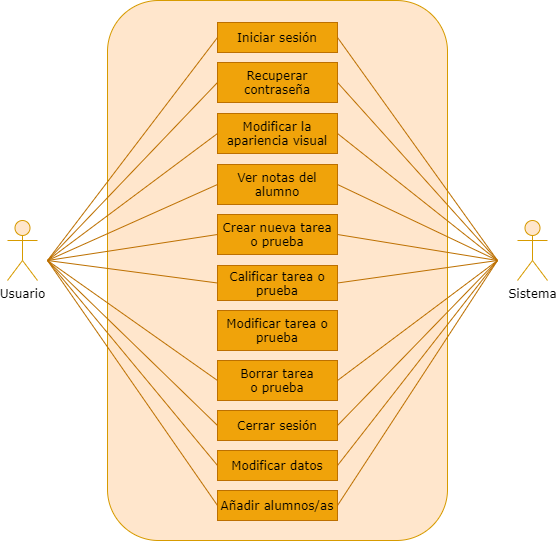
\includegraphics[width=1\linewidth]{figs/diagramacdu.png}
\caption{Diagrama de casos de uso de la aplicación.}
\label{Fig:diagramacdu}
\end{figure}


\subsection{Prueba de usabilidad}
\label{sub:pruebausabilidad}
Con el fin de llevar a cabo correctamente el requisito no funcional de usabilidad, se ha decidido realizar una prueba de usabilidad de forma voluntaria con 34 profesores y maestros entre los que se incluyen docentes de Educación Primaria, Educación Secundaria y universidad.

A estos docentes se les proporcionó un vídeo explicativo mostrando y explicando las funcionalidades de la aplicación con el resultado obtenido de este trabajo, y un cuestionario de 10 preguntas para recoger sus opiniones realizado con Google Forms.

De las 10 preguntas, la primera pregunta sirve para que el encuestado dé su consentimiento para realizar el cuestionario, la segunda y la tercera son preguntas para obtener su perfil (género y trabajo), la cuarta [\ref{Fig:pregunta4}] y la quinta [\ref{Fig:pregunta5}] son preguntas que utilizan respuestas tipo Likert de 5 niveles, la sexta, séptima y octava son preguntas de respuesta abierta donde el encuestado puede mostrar su opinión y la novena [\ref{Fig:pregunta9}] y la décima preguntan si estarían interesados en recibir actualizaciones de la aplicación y seguir su desarrollo.

\begin{figure}[h]
\centering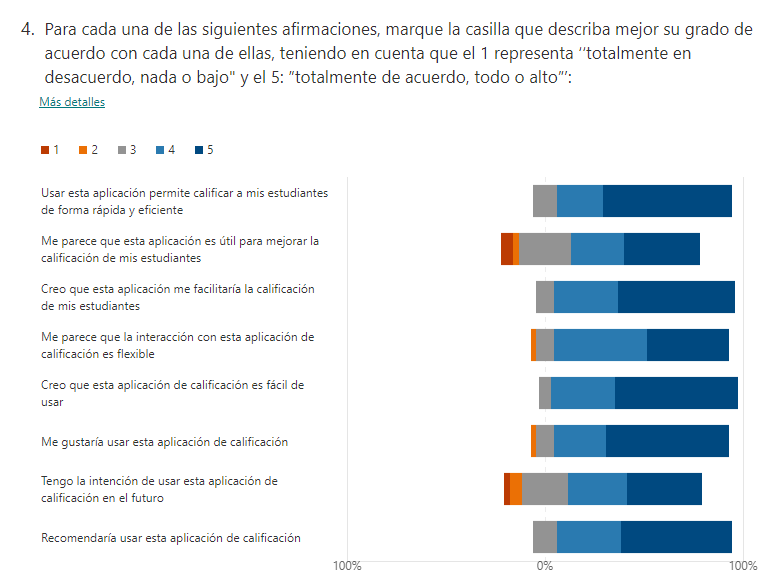
\includegraphics[width=1\linewidth]{figs/pregunta4.png}
\caption{Pregunta 4 del cuestionario.}
\label{Fig:pregunta4}
\end{figure}

\begin{figure}[h]
\centering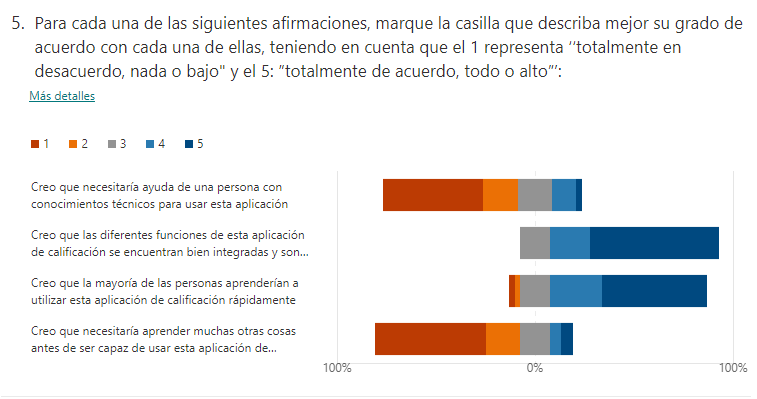
\includegraphics[width=1\linewidth]{figs/pregunta5.png}
\caption{Pregunta 5 del cuestionario.}
\label{Fig:pregunta5}
\end{figure}

\begin{figure}[h]
\centering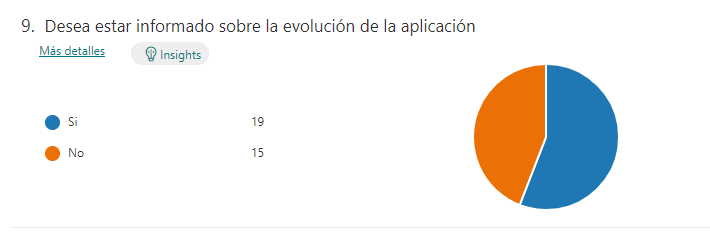
\includegraphics[width=1\linewidth]{figs/pregunta9.png}
\caption{Pregunta 9 del cuestionario.}
\label{Fig:pregunta9}
\end{figure}

A continuación se realiza un pequeño análisis sobre el cuestionario.

Los resultados han sido generalmente favorables. Considerando, en la cuarta pregunta, que un 4 o un 5 son respuestas aceptables, se puede observar que al 64,7\% de los encuestados les parece útil la aplicación desarrollada para mejorar la forma en la que califican a sus estudiantes, y al 88.3\% les gustaría poder llegar a usarla.

En la quinta pregunta también encontramos resultados contundentes. Solo el 11,8\% de los encuestados considera que necesitaría formación previa para usar la aplicación correctamente respecto al 73,5\% que no creen que fueran a tener ningún problema.

Algunos comentarios de los encuestados cuando se les preguntó por los puntos fuertes de la aplicación son:
\begin{quote}
\textit{\"Sencillez y rapidez. Quizá lo más interesante sea la claridad a la hora de ofrecer la información global, pero sobre todo las medias por evaluación. Lo mejor es su interacción y la posibilidad de exportarlo a una hoja Excel convencional.\"}
\end{quote}

\begin{quote}
\textit{\"Puedes añadir y eliminar alumnos/as fácilmente y tienes toda la información de tus alumnos/as a un golpe de ratón.\"}
\end{quote}

\begin{quote}
\textit{\"Visualización rápida, flexibilidad en la interacción.\"}
\end{quote}

También se muestran algunos de los comentarios de los encuestados cuando se les preguntó si querían mostrar su opinión:
\begin{quote}
\textit{\"Me sorprendió la posibilidad de uso para daltónicos, entre los que me incluyo.\"}
\end{quote}

\begin{quote}
\textit{\"No sé si puede usarse con un sistema operativo diferente de Windows, pero sería una ventaja que pudiera usarse con Linux y LibreOffice. Espero que sea así.\"}
\end{quote}

\begin{quote}
\textit{\"Me gustaría utilizarla y ver personalmente su eficacia.\"}
\end{quote}

Para finalizar, comentar que varios de los puntos débiles de la aplicación se han tenido en cuenta y se han mencionado en la sección \ref{sec:trabajofuturo}: Propuestas de trabajo futuro. Sin embargo, como muestra, los comentarios generales más críticos han sido referentes a la interfaz gráfica de la aplicación:

\begin{quote}
\textit{\"Me parece una aplicación útil y completa, pero el aspecto visual podría estar más trabajado.\"}
\end{quote}

\begin{quote}
\textit{\"Como profesora de primaria me gustaría incorporar dibujos o 'caritas'\".}
\end{quote}

\begin{quote}
\textit{\"Hay que introducir demasiados datos, creo que es más útil en instituto que en universidad, donde se hacen menos pruebas y no hace tanta falta una herramienta de este tipo.\"}
\end{quote}

Para finalizar esta sección, se comenta que se hizo una pequeña prueba de usabilidad con una persona daltónica mostrándole primero los colores por defecto y después los colores elegidos para el 'Modo daltónicos'. Afirmó que solo el segundo conjunto de colores era fácilmente distinguible.

\section{Decisiones de diseño e implementación}
En esta sección se describirán algunas de las decisiones que se han tomado respecto al diseño de la aplicación que pueden ser de interés.

\subsection{Procedencia de los iconos e imágenes de la aplicación}
Los iconos de una aplicación son un arma de doble filo: pueden guiar al usuario por las tareas que quiere realizar o confundirlo si la funcionalidad asociada al icono no es clara o, directamente, es incoherente.

Para implementar iconos en esta aplicación se han decidido usar las convenciones de las aplicaciones modernas: una imagen de un disquete para los botones de guardar, una cruz roja para cancelar, un icono de encendido para cerrar sesión...

Sin embargo, para las funcionalidades específicas, se han diseñado la mayoría de los iconos e imágenes mediante la aplicación Procreate [\ref{sub:procreate}]. Los iconos que no se han diseñado y se han descargado de Internet han sido el disquete \cite{disquete}, el icono de Microsoft Excel \cite{excelicon} y el icono de la papelera \cite{iconsforfree}.

\subsection{Opciones especiales para personas con daltonismo}
A la hora de implementar las opciones de colores para la interfaz, accesibles mediante la ventana de inicio de sesión, ha sido muy importante tener en cuenta todas las combinaciones de colores de manera que, aun eligiendo tonos parecidos, se pudiera seguir leyendo correctamente.

La investigación que se llevó a cabo probando diferentes tonalidades  llevó a pensar que, efectivamente, hay personas que no distinguen bien colores que, a primera vista, son muy diferentes, como pueden ser el verde y el rojo asignados a las calificaciones aprobado y suspenso, respectivamente. Esta condición se llama daltonismo, que es una alteración de origen genético que impide identificar correctamente los colores. Uno de los tipos de daltonismo más comunes es la deuteranopia, razón por la cual se incluyó en las opciones de personalización un "modo para daltónicos".

Esta opción especial modifica los colores de aprobados y suspensos para que sean colores fácilmente reconocibles para personas con esta condición (ver figura \ref{Fig:appdaltonicos}.

\begin{figure}[h]
\centering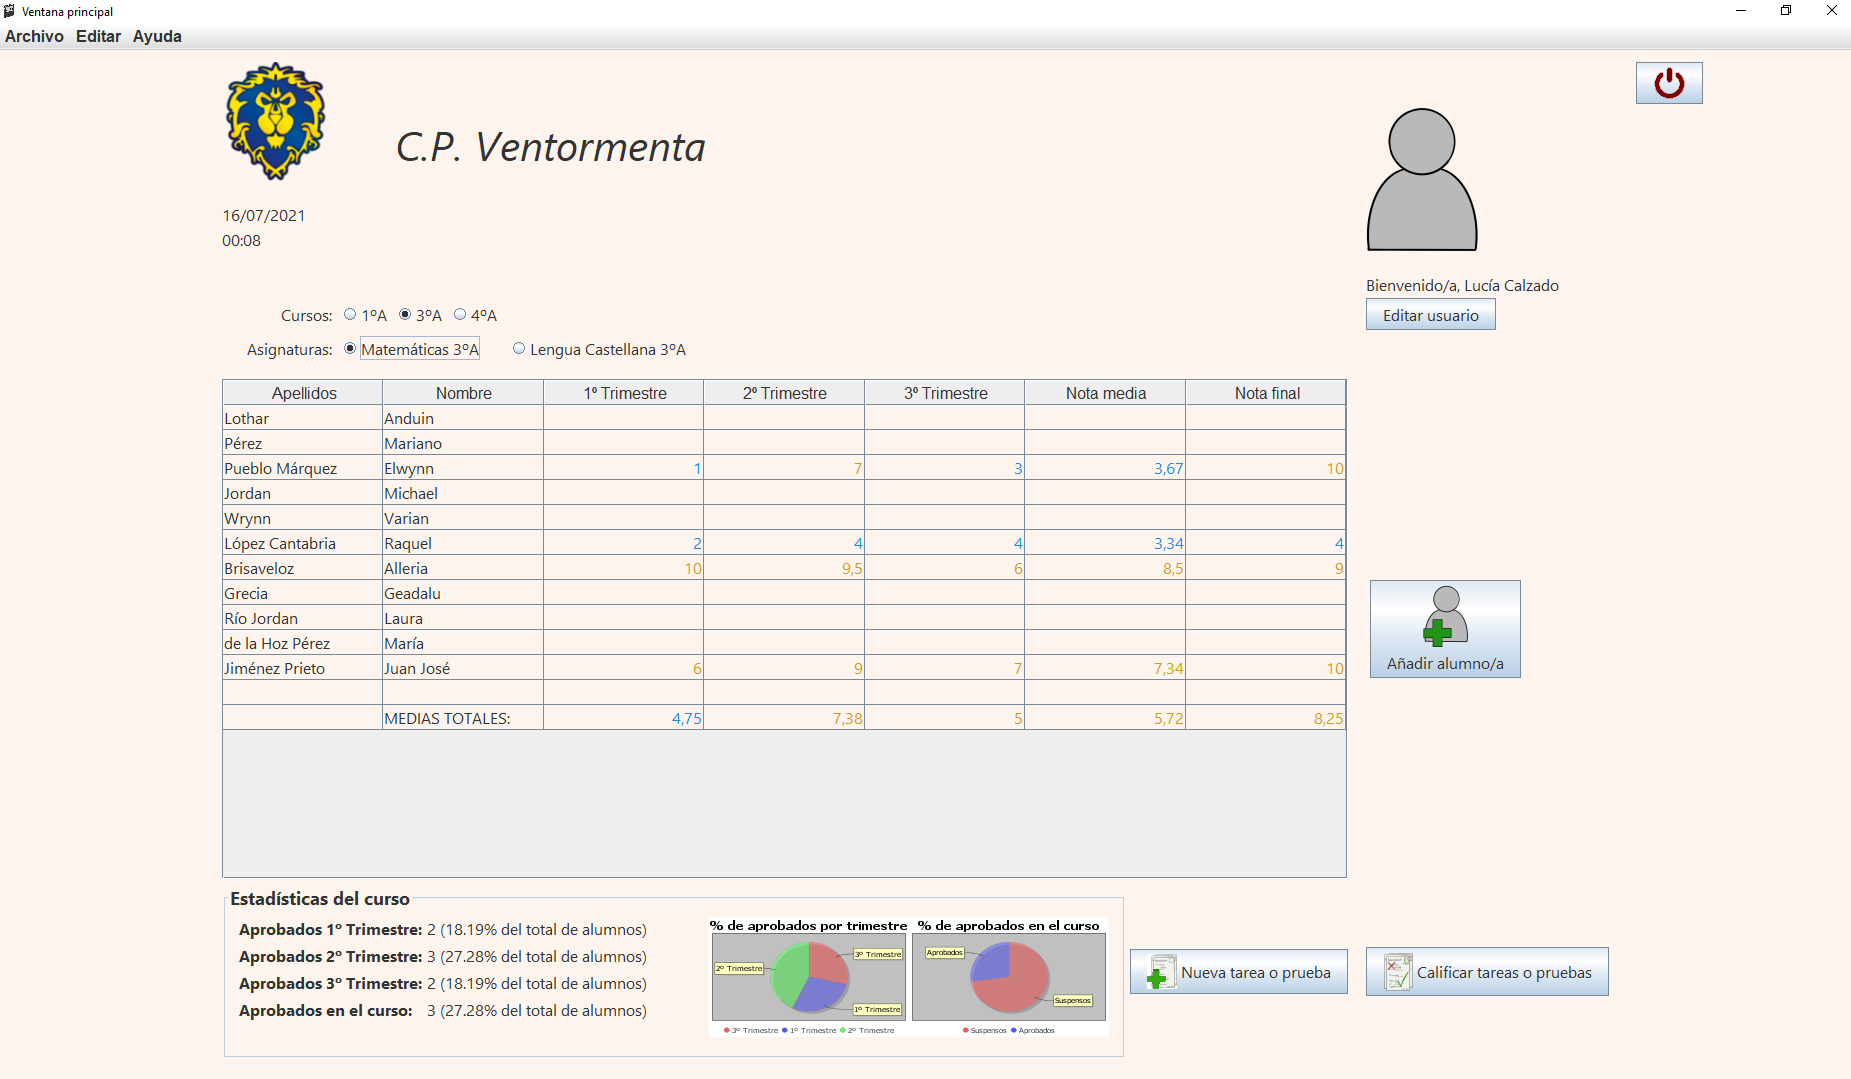
\includegraphics[width=1\linewidth]{figs/appdaltonicos.png}
\caption{Visualización de la pantalla principal con el modo daltónicos activado.}
\label{Fig:appdaltonicos}
\end{figure}

\subsection{Optimización del código}
\label{sub:optimizarcodigo}
El código, si bien no posee algoritmos optimizables, se ha investigado y diseñado de forma que se ejecuten las instrucciones mínimas posibles, cuando ha sido posible.

Además se ha primado el uso de diccionarios como estructura principal de almacenamiento de datos, en concreto de los HashMaps, la estructura de diccionario de Java más rápida para el alcance del problema \cite{hashmap}.

El tiempo de acceso de las operaciones añadir, borrar y buscar es \textit{O(1)}. Estas son las operaciones que se han usado en el código. Además, la única casuística en la que un HashMap pudiera dar problemas de rendimiento sería si tuviera demasiados datos dentro: las operaciones se volverían más lentas. Esto también se ha evitado en la solución propuesta, donde el número máximo de elementos de cualquiera de estas estructuras es el número de alumnos en una asignatura.

\section{Resultado del desarrollo}
En esta sección se muestra el resultado del desarrollo de la aplicación de este documento mediante capturas de pantalla de la solución, acompañadas de una descripción.

En el Anexo 1 se pueden encontrar diagramas de secuencia de los casos de uso más interesantes.

\subsection{Inicio de sesión}
Se ha desarrollado una ventana para que el usuario inicie sesión (ver figura \ref{Fig:login}). Es la primera ventana que se encuentra al ejecutar el programa.

\begin{figure}[h]
\centering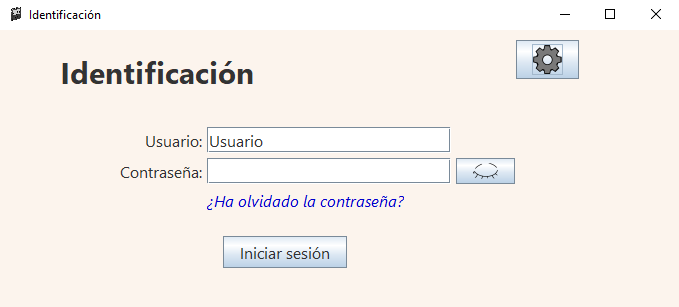
\includegraphics[width=1\linewidth]{figs/login.png}
\caption{Pantalla de inicio de sesión.}
\label{Fig:login}
\end{figure}

Esta ventana permite al usuario acceder a las opciones del programa haciendo clic en la rueda de opciones, e iniciar sesión en la aplicación con su DNI y una contraseña asociada. En la figura \ref{Fig:loginopciones} se pueden ver las diferentes opciones de personalización que se ofrecen:
\begin{itemize}
	\item \textbf{Cambio del tamaño de la letra}, seleccionando entre 5 diferentes tamaños de letra.
	\item \textbf{Colores para las notas aprobadas, suspensas y el fondo de la aplicación}. Hay también 5 opciones para los colores de las notas, que son colores sólidos y fuertes, y otras 5 para el fondo, colores pastel que permiten el contraste de los demás elementos de la ventana.
	\item \textbf{Modo oscuro}. Este modo modifica toda la interfaz gráfica, cambiando el contraste con un fondo negro y letras blancas. Esta opción de diseño se llevó a cabo debido a que a medida que va pasando el tiempo, el 'modo nocturno' o 'modo oscuro' de los dispositivos y aplicaciones se vuelve más popular.
	\item \textbf{Modo daltónicos}. Este modo bloquea la posibilidad de cambiar los colores de aprobados y suspensos, poniendo dos colores que son fácilmente distinguibles para la mayoría de personas con daltonismo.
\end{itemize}

\begin{figure}[h]
\centering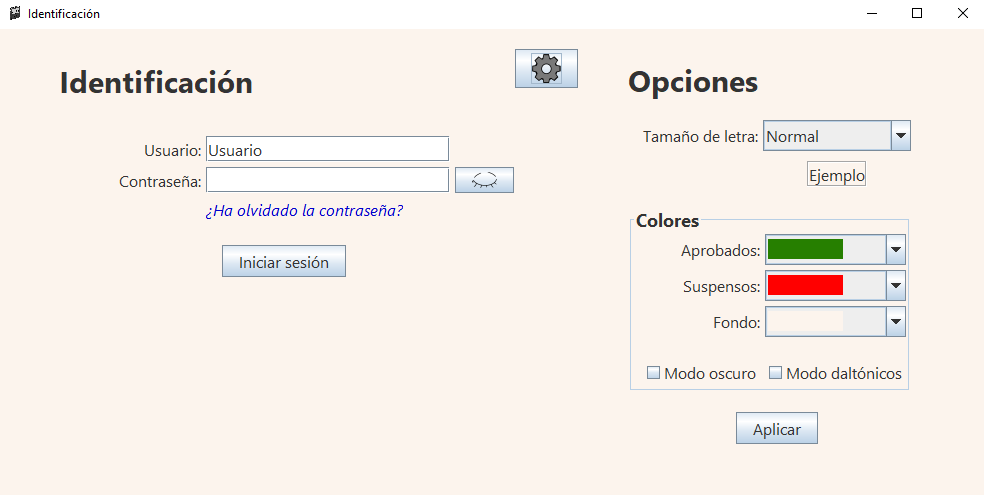
\includegraphics[width=1\linewidth]{figs/loginopciones.png}
\caption{Pantalla de inicio de sesión con opciones.}
\label{Fig:loginopciones}
\end{figure}

Esta ventana también contiene un botón con un ojo cerrado que, al hacerle clic, se abre y muestra la contraseña, y una opción de recuperado de contraseña por si el usuario se olvidara de ella.


\subsection{Ventana principal}
Esta ventana es el centro de operaciones de la aplicación, y desde aquí se puede navegar a todas sus características y funcionalidades, de las que se habla en las siguientes secciones. Esta ventana se puede ver en la figura \ref{Fig:ventanaprincipal}.

\begin{figure}[h]
\centering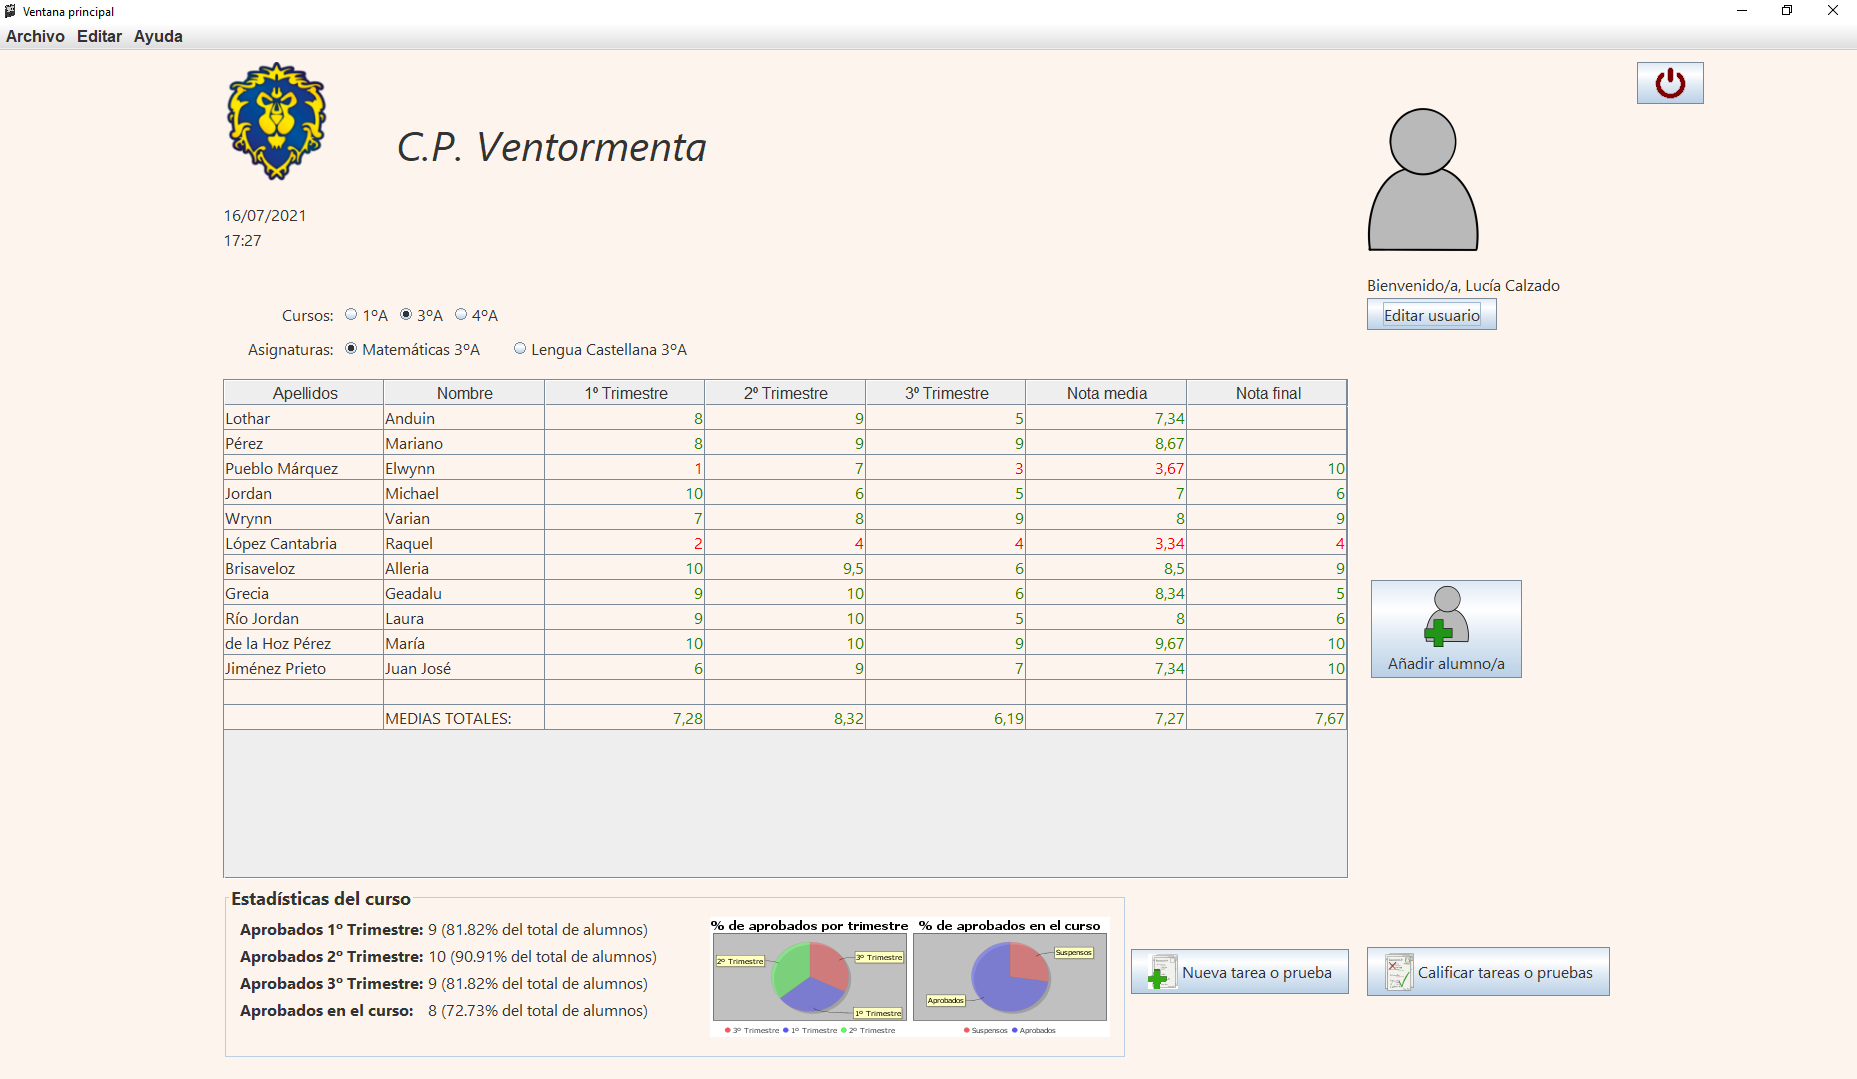
\includegraphics[width=1\linewidth]{figs/ventanaprincipal.png}
\caption{Ventana principal de la aplicación.}
\label{Fig:ventanaprincipal}
\end{figure}

En el menú de arriba se puede cerrar sesión en Archivo>Cerrar sesión, añadir un alumno o varios desde el menú Editar>Alumnos y acceder al manual de ayuda en Ayuda>Manual de ayuda, así como visualizar una pequeña ventana 'Acerca de...' que muestra los datos personales de la desarrolladora de este trabajo.

En la parte de arriba de la ventana vemos el logotipo y el nombre del Centro que está usando la aplicación, así como la fecha y la hora del día actual. 

En el centro, el usuario puede elegir el curso y la asignatura para los que desea hacer los trámites, y aparece una tabla con los alumnos asignados y sus notas finales para cada trimestre, una nota media de los tres trimestres y una nota final. Cabe notar que las notas tienen colores (que se pueden personalizar en las opciones de la ventana de Inicio de sesión) dependiendo de si el trimestre está aprobado o suspenso. El usuario también puede consultar la fecha de cierre de actas para cada trimestre manteniendo el ratón por encima del nombre de cada trimestre en la tabla. Esta información se muestra mediante un \textit{tooltip}.

En la última fila de la tabla también hay un cálculo de medias, esta vez por trimestre y no por alumno.

Debajo de la tabla se ven las estadísticas de la asignatura: el número de aprobados por trimestre y en total en el curso, así como dos diagramas de quesitos mostrando los datos mencionados anteriormente: uno para los aprobados por cada trimestre, para representar de manera visual qué trimestre ha sido el más exitoso, y uno de los alumnos aprobados en todo el curso, para representar el éxito del curso en general.

A la derecha de estas estadísticas están los accesos a las funcionalidades de crear una nueva tarea y calificar a los alumnos en las tareas existentes, así como la de añadir un alumno nuevo a la asignatura.

Por último, arriba a la derecha se encuentran los datos del maestro: su nombre y su fotografía, y el acceso a la funcionalidad de modificar los datos del usuario, así como el botón de cerrar sesión, arriba a la derecha.


\subsection{Editar usuario}
Mediante el botón Editar usuario en la pantalla principal, se accede a la ventana de modificar los datos del usuario: el nombre mediante el que se dirige a él la aplicación, una fotografía personal y la contraseña de inicio de sesión. Esta ventana se puede ver en la figura \ref{Fig:datospersonales}.

\begin{figure}[h]
\centering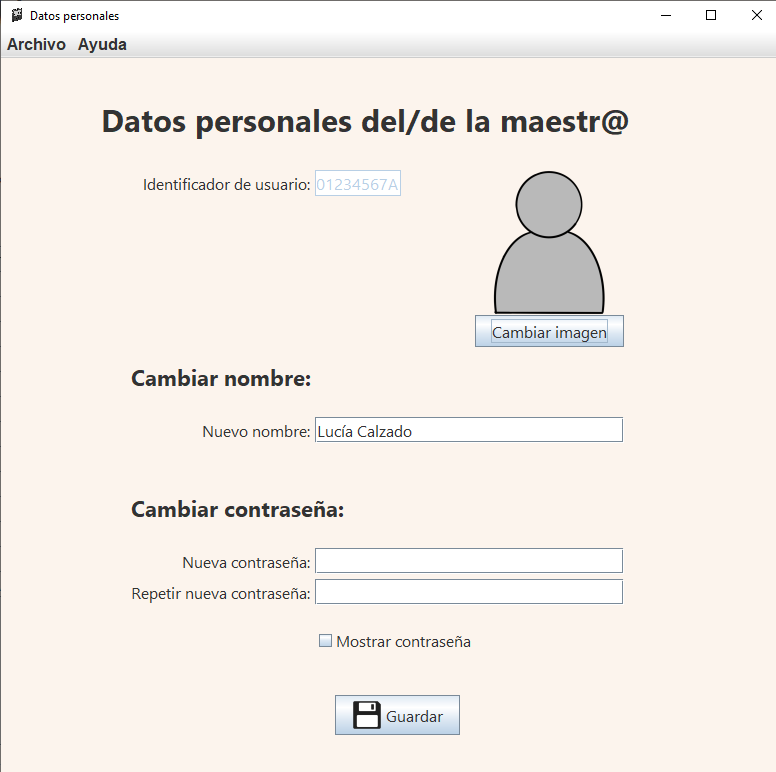
\includegraphics[width=0.5\linewidth]{figs/datospersonales.png}
\caption{Ventana para modificar los datos personales del usuario.}
\label{Fig:datospersonales}
\end{figure}

\subsection{Añadir alumno}
La aplicación permite añadir alumnos de dos maneras. Se puede añadir un solo alumno rellenando un formulario (ver figura \ref{Fig:añadiralumno}), accesible tanto el botón Añadir alumno/a como en el menú Editar>Alumnos de la ventana principal.

\begin{figure}[h]
\centering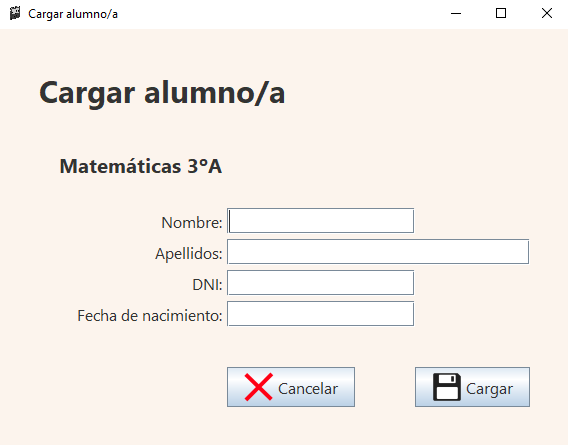
\includegraphics[width=0.5\linewidth]{figs/cargaralumno.png}
\caption{Formulario para añadir un alumno.}
\label{Fig:añadiralumno}
\end{figure}

La segunda opción es añadir varios alumnos cargando un Excel con sus datos: nombre, apellidos, DNI y fecha de nacimiento. Esta opción es únicamente accesible en la ventana principal, mediante el menú Editar>Alumnos.

La aplicación añade los alumnos teniendo en cuenta la asignatura desde la que se ha llamado la funcionalidad. Si la asignatura es troncal, quiere decir que los alumnos están siendo asignados a un curso entero, porque las asignaturas troncales son de carácter obligatorio. Si, por el contrario, son añadidas a una asignatura optativa, solo se añadirán a esa asignatura optativa, no al curso, debido a que las asignaturas optativas son opcionales.

\subsection{Crear nueva tarea}
Una de las dos funcionalidades principales de la aplicación es la de crear una tarea (o prueba) nueva (ver figura \ref{Fig:creartarea}). Esta característica es accesible mediante el botón 'Nueva tarea o prueba' de la ventana principal, una vez se ha seleccionado una asignatura.

\begin{figure}[h]
\centering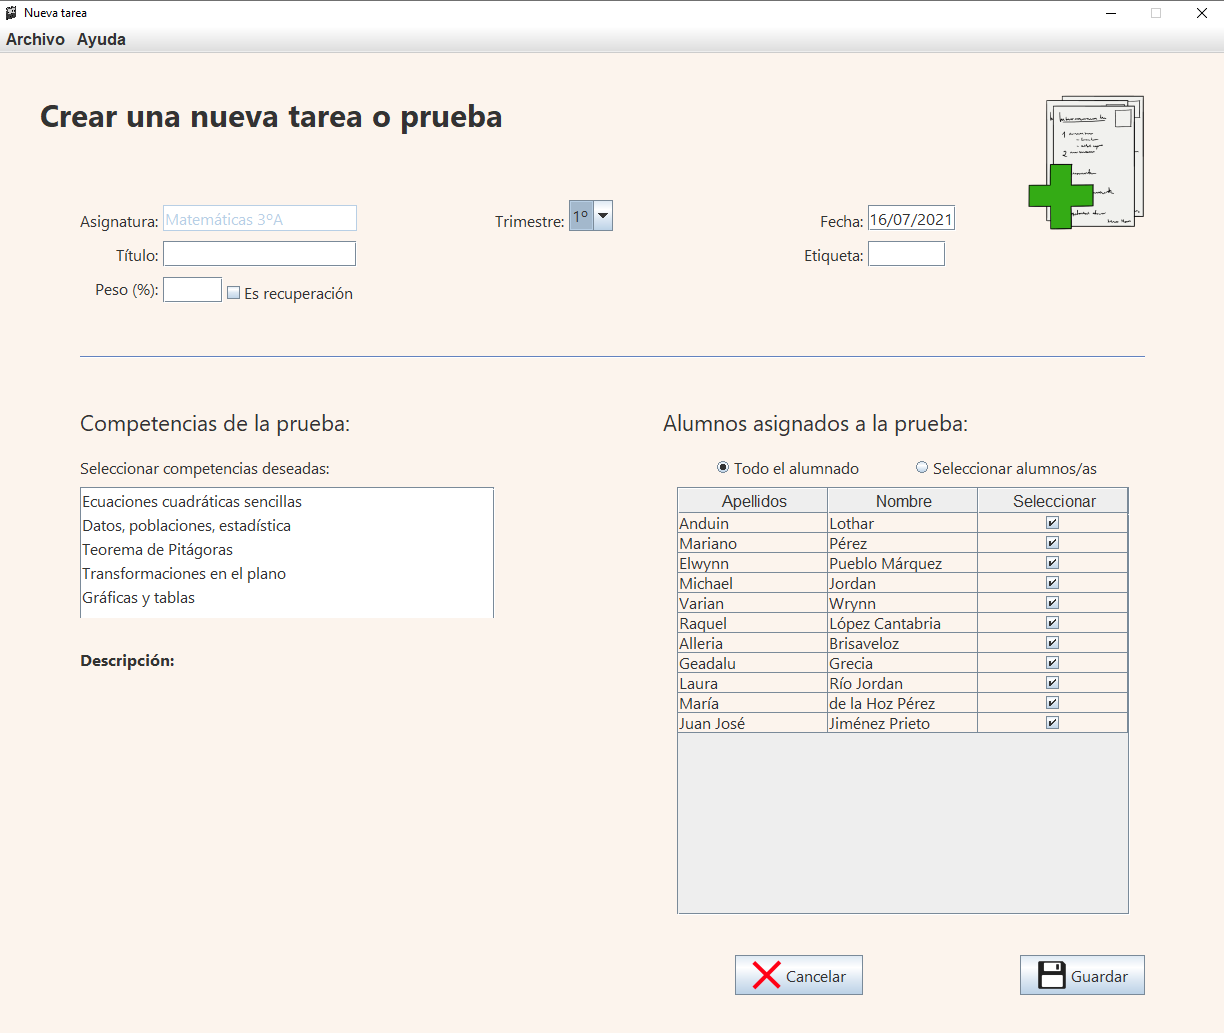
\includegraphics[width=1\linewidth]{figs/creartarea.png}
\caption{Formulario para crear una tarea (o prueba) nueva.}
\label{Fig:creartarea}
\end{figure}

La ventana consta de un formulario que tiene que rellenar el usuario para crear una tarea nueva. A continuación se muestra una breve descripción de los campos:
\begin{itemize}
	\item \textbf{Título:} este es el título que tiene la prueba, usado para consultar las notas en el módulo Calificar tareas o pruebas.
	\item \textbf{Trimestre:} el trimestre para el que se crea la prueba. Es importante para posterior ordenación y muestra de las pruebas por trimestres.
	\item \textbf{Peso:} el peso de la prueba dentro del trimestre, o el porcentaje de la nota final del trimestre que corresponde a esa prueba.
	\item \textbf{Fecha:} la fecha en la que se llevará a cabo la prueba.
	\item \textbf{Etiqueta:} un pequeño título único para la prueba. Debe tener como máximo 5 caracteres.
	\item \textbf{Competencias:} se deben seleccionar las competencias asignadas a la prueba de la lista de competencias. En el apartado Descripción, salen las descripciones asignadas a cada competencia.
	\item \textbf{Alumnos asignados:} debido a que algunas pruebas podrían no ser opcionales o ser exámenes de recuperación, se pueden elegir los alumnos a los que se les quiere asignar la prueba.
\end{itemize}

Cuando se hace clic en el botón de guardar, la prueba se almacena en la base de datos con los datos del formulario.


\subsection{Calificar tareas}
La segunda de las funcionalidades principales de la aplicación es la de calificar las tareas creadas mediante el módulo anterior (ver figura \ref{Fig:calificartarea}). Para acceder a este módulo, se debe hacer clic en el botón 'Calificar tareas o pruebas' de la ventana principal, una vez se ha seleccionado una asignatura.

\begin{figure}[h]
\centering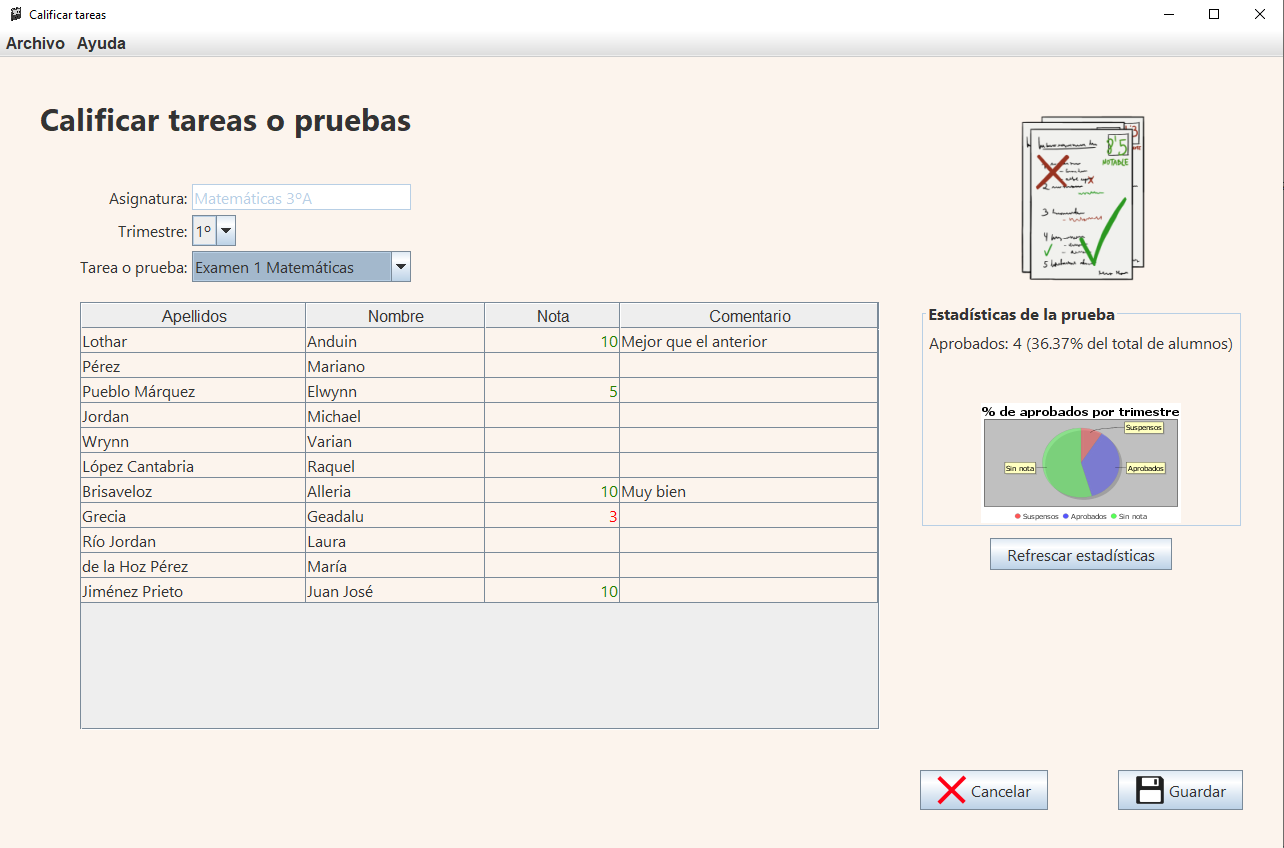
\includegraphics[width=1\linewidth]{figs/calificartareas.png}
\caption{Ventana para calificar las tareas (o pruebas) creadas.}
\label{Fig:calificartarea}
\end{figure}

En esta ventana, se puede elegir el trimestre de la prueba que se va a calificar, y después la misma prueba. Esto cargará una tabla con todos los alumnos de la asignatura, una columna para calificarlos y otra para asignarles un comentario, si el docente considera oportuno.

Si un alumno no tiene que realizar una prueba, por defecto, en el comentario saldrá escrito \textit{"No tiene que hacer la prueba."}. 

A la derecha de la tabla se puede observar otro panel de estadísticas, que muestran el porcentaje de alumnos aprobados en la prueba.

Cuando se haya calificado a los alumnos, al hacer clic en el botón de guardar, se guardarán los cambios en la base de datos.

\subsection{Informe del alumno}
Esta ventana muestra todas las notas, tanto de pruebas como finales, de un alumno en particular (ver figura \ref{Fig:informealumno}). Es accesible haciendo clic en el nombre o apellidos de un alumno en la tabla de la ventana principal.

\begin{figure}[h]
\centering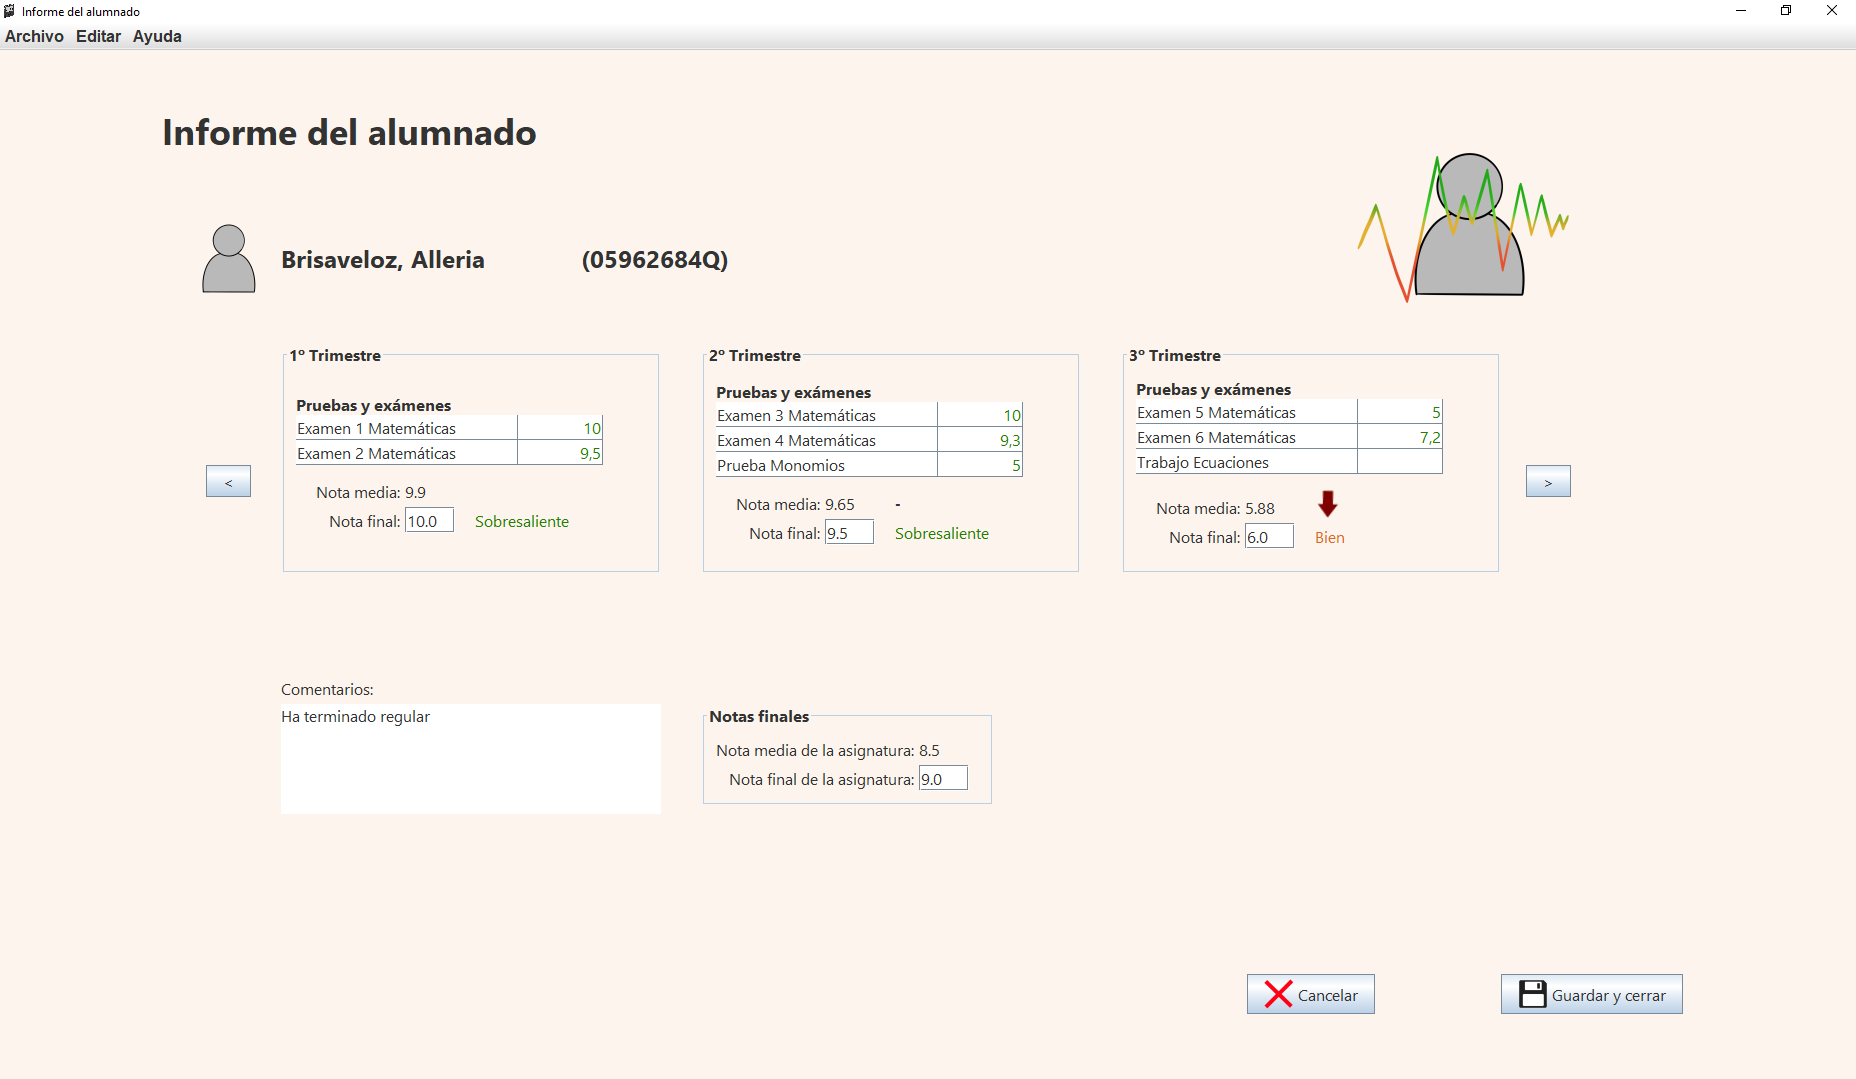
\includegraphics[width=1\linewidth]{figs/informealumno.png}
\caption{Ventana del informe general del alumno.}
\label{Fig:informealumno}
\end{figure}

En la parte de arriba está el nombre y apellidos del alumno, así como su DNI y su fotografía personal.

En el centro de la ventana hay tres tablas que corresponden a los tres trimestres. Cada tabla contiene todas las pruebas de ese trimestre, junto con la nota del alumno. Si se deja el ratón por encima de la nota, se muestra el comentario (si lo hubiera), de la misma mediante un \textit{tooltip}. Debajo de la tabla aparece la media de las notas de las pruebas y la nota final de ese trimestre.

La característica más interesante de esta ventana es la información que se obtiene de cada trimestre:
\begin{itemize}
	\item{Color de las notas según la calificación,} de la misma forma que en la ventana principal.
	\item{Calificaciones}. Las calificaciones (insuficiente, suficiente, bien, notable y sobresaliente) salen según el usuario introduce la nota final en cada trimestre.
	\item{Comparaciones con trimestres anteriores} mediante flechas en el segundo y tercer trimestre. Si la parte entera de la media del trimestre es mayor que la del trimestre anterior, aparece una flecha verde. Si es menor, aparece una flecha roja. Si es igual, no aparece nada.
\end{itemize}

Para finalizar, en la parte de abajo, el usuario puede introducir un comentario general del alumno para esa asignatura, y asignarle una nota final.

\subsection{Informe del trimestre}
Mediante esta vista se pueden ver las notas de todos los alumnos de un trimestre y gestionar las pruebas del mismo. Se puede acceder a ella haciendo clic en el nombre de un trimestre en la ventana principal.

\begin{figure}[h]
\centering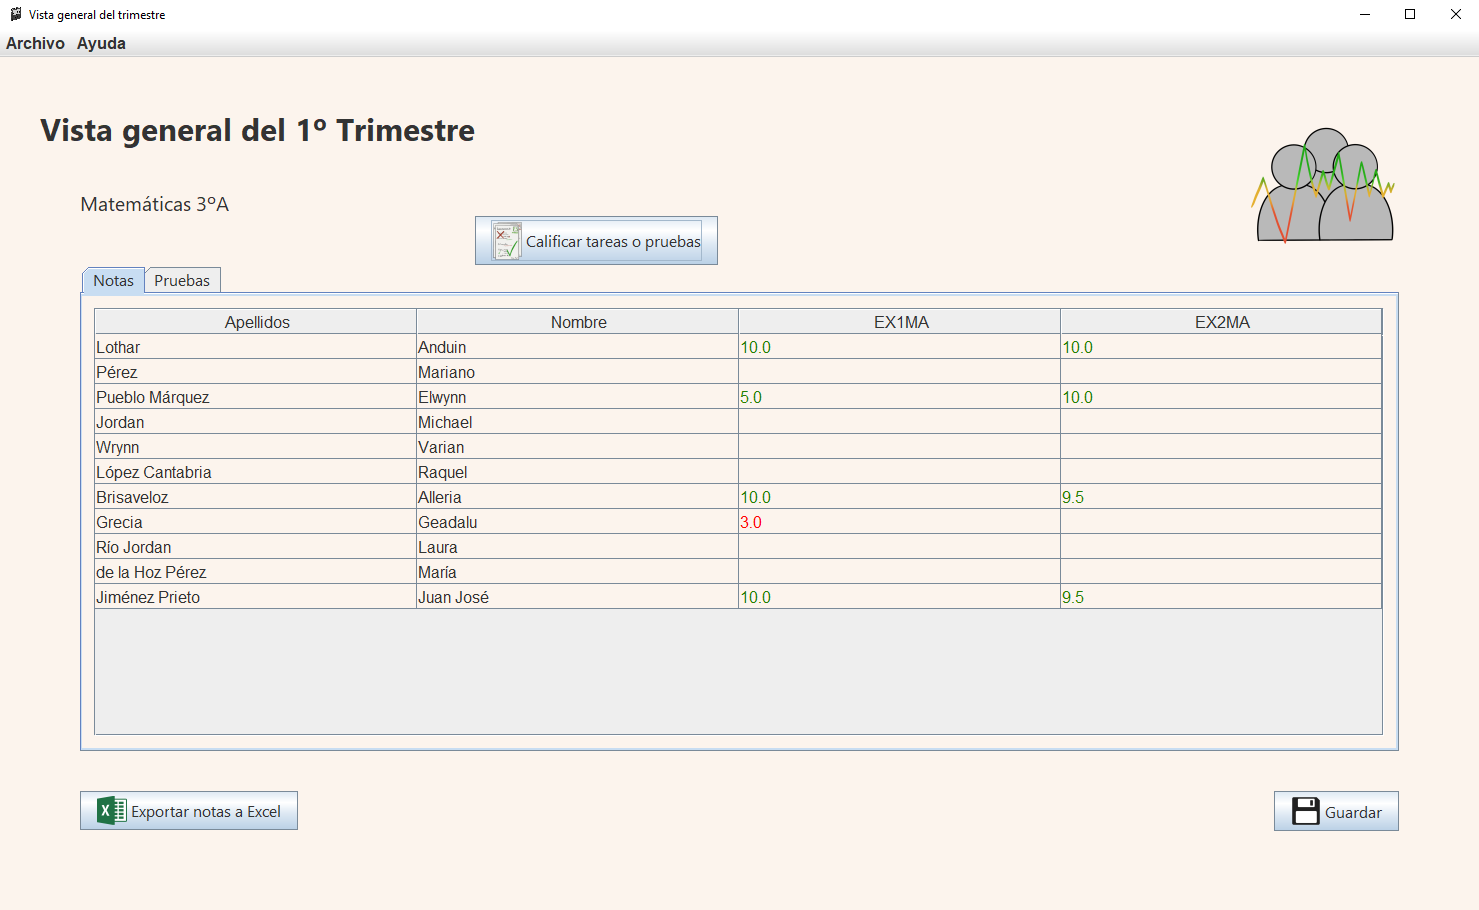
\includegraphics[width=1\linewidth]{figs/informetrimestre.png}
\caption{Primera pestaña de la ventana del informe por trimestre.}
\label{Fig:informetrimestre}
\end{figure}

Esta ventana está dividida, como hemos mencionado, en dos partes: la primera muestra una tabla informativa con todas las notas de las pruebas del trimestre elegido (ver figura \ref{Fig:informetrimestre}). En caso de que un alumno no tuviera que hacer la prueba, en la casilla saldría un guión '-'. 

\begin{figure}[h]
\centering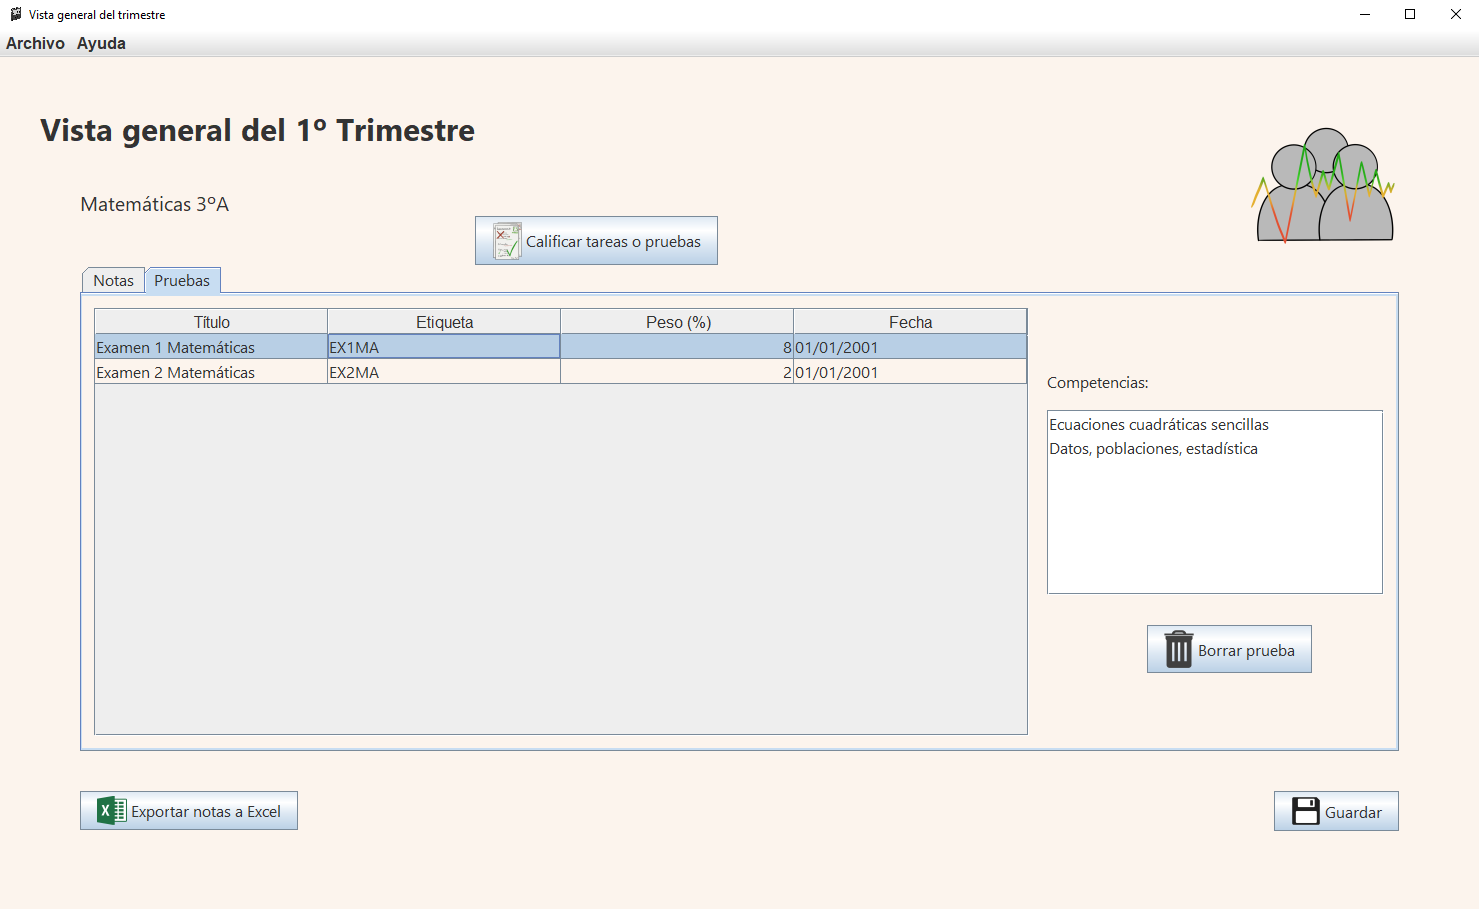
\includegraphics[width=1\linewidth]{figs/informetrimestre2.png}
\caption{Segunda pestaña de la ventana del informe por trimestre.}
\label{Fig:informetrimestre2}
\end{figure}

La segunda parte, accesible mediante la pestaña "Pruebas", presenta, en una tabla, los datos de las pruebas que se han introducido mediante el formulario de crear una nueva prueba, con posibilidad de edición (ver figura \ref{Fig:informetrimestre2}). Además, al seleccionar una prueba, a la derecha aparecerán las competencias asignadas a la misma y un botón para borrar la prueba del sistema, que borrará también las notas de los alumnos, si las tenían, y refrescará las dos tablas de la ventana.

\subsection{Manual de ayuda}
Existe un manual de ayuda, accesible por todas las ventanas desde el menú Ayuda>Manual de ayuda, que el usuario puede consultar en caso de duda sobre alguna funcionalidad.

Este manual se abre directamente por la página de la ventana desde la que se llama, y ofrece información detallada sobre lo que se puede hacer en cada ventana.

Se puede ver esta ventana en la figura \ref{Fig:ayuda}.

\begin{figure}[h]
\centering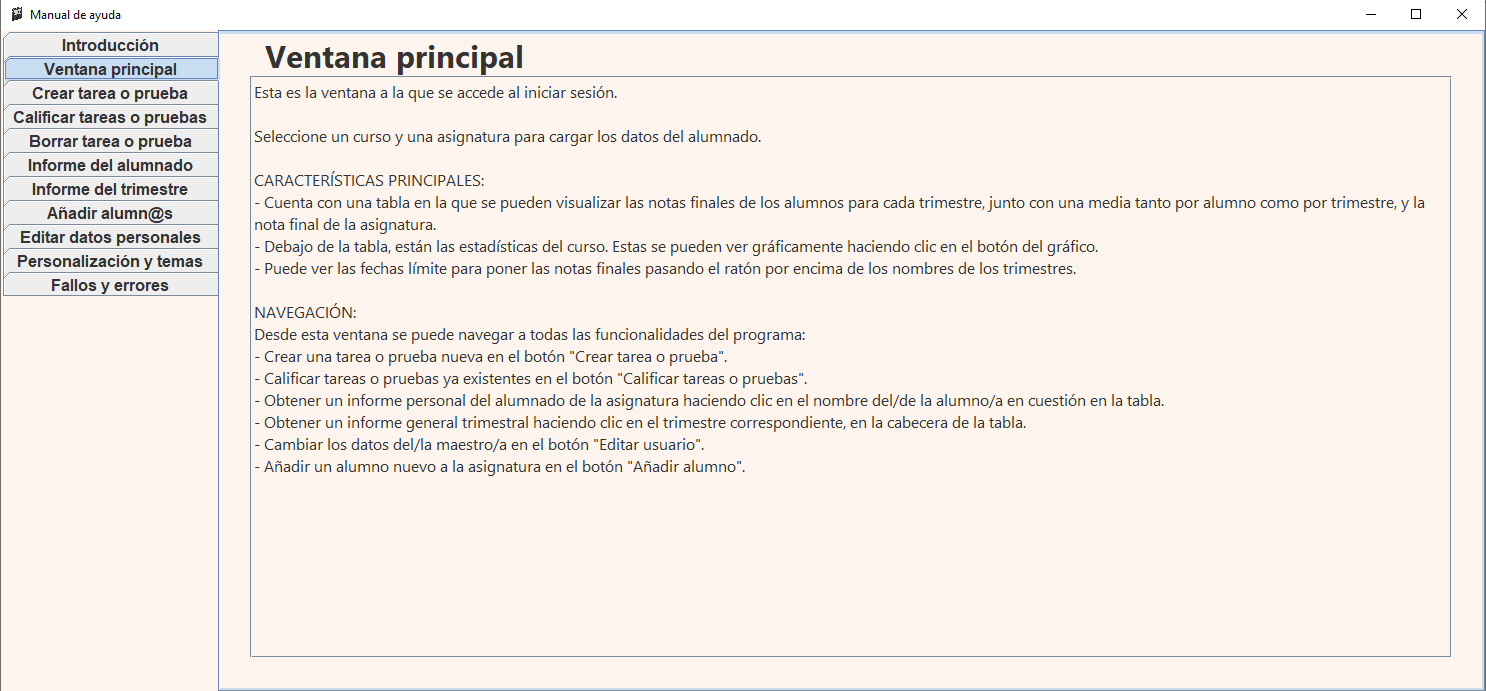
\includegraphics[width=1\linewidth]{figs/ayuda.png}
\caption{Ventana con el manual de ayuda.}
\label{Fig:ayuda}
\end{figure}